\chapter{Details about the parton-level simulations}
\label{chap:Appendix:TopPartons}




%%%%%%%%%%%%%%%%%%%
%           Developing TopPartons       %
%%%%%%%%%%%%%%%%%%%
\section{Software package for parton-level information}
\label{sec:ChaptH:Sig:truth:TopPartons}
%\paragraph{TopPartons}\mbox{}\\
The \texttt{TopPartons} package performs the analysis of the parton-level truth information.
For all particles except the ones in the final state, the information stored in the NTuples
corresponds to the after-final-state radiation\footnote{The after FSR corresponds to the
 particle right before decaying to its children. In contrast to the FSR, the initial-state radiation (ISR) refers 
 to the particle state when it was produced.The ISR is always more energetic than the FSR since as the
 particle travels it radiates energy.} (FSR).  For the final state particles, the ISR information is saved.
For each particle, the PDG-ID, \pT, $\eta$, $\phi$ and mass are stored. Additionally, some of the $\tau$ related
variables contain information on whether $\tau$ decays hadronically or leptonically.  If the $\tau$ decays to a 
light lepton, it stores the PDG-ID of that lepton and if it decays hadronically it stores the PDG-ID of the \PWm for $\tau^-$ 
and the \PWp for $\tau^+$.


\paragraph{Decay of the Higgs boson and the top quark}\mbox{}\\
First of all, the code searches for the Higgs boson by looking at the PDG-ID of the truth 
particles. Then, it takes into account all the considered Higgs-boson decays 
and demands that it has exactly two children. 
%This is done using the functions \texttt{HiggsAndDecay} of \texttt{CalcThqPartonHistory.cxx} .
The FSR state of the Higgs boson is stored and its children are studied
If the Higgs boson does not decay into 
$\PWplus\PWminus$, $\Ptauon \APtauon$ or $\PZ\PZ$, the event is discarded. 
To fill the truth variables it is also required that the top quark decays into $\PW$$\Pbottom$.


% Spectator quark ambiguity at NLO 
\paragraph{Spectator-quark ambiguity at NLO}\mbox{}\\
The script identifies the
spectator quark, i.e. the quark that comes from the hard-scattering process.
At NLO, the spectator quark is not well defined from first principles at the parton level 
and, therefore, there would be no way that one can do a proper parton assignment with NLO generators.

To properly select the spectator light-quark, firstly the top quark is searched and then its parent found\footnote{%
Note that in \PYTHIA the intermediate quarks are left out so the parent of the top would be the gluon and $q$ in the 
diagram of Figure~\ref{fig:tHq:TruthFeyman:HfromW}.
The children of the gluon are the $b$-quark, the top and $q'$.}. 
The spectator quark is selected at parton level from among the light quarks after 
the QED and QCD radiations that are not products of the top quark decay. 
In case of ambiguities arising from ISR, the spectator quark that minimises the \pT of 
the combined spectator quark and top quark system is chosen.
%   If there are several light-quark candidates, the one with highest \pT is taken as spectator. 

\begin{figure}[htbp!]
\centering
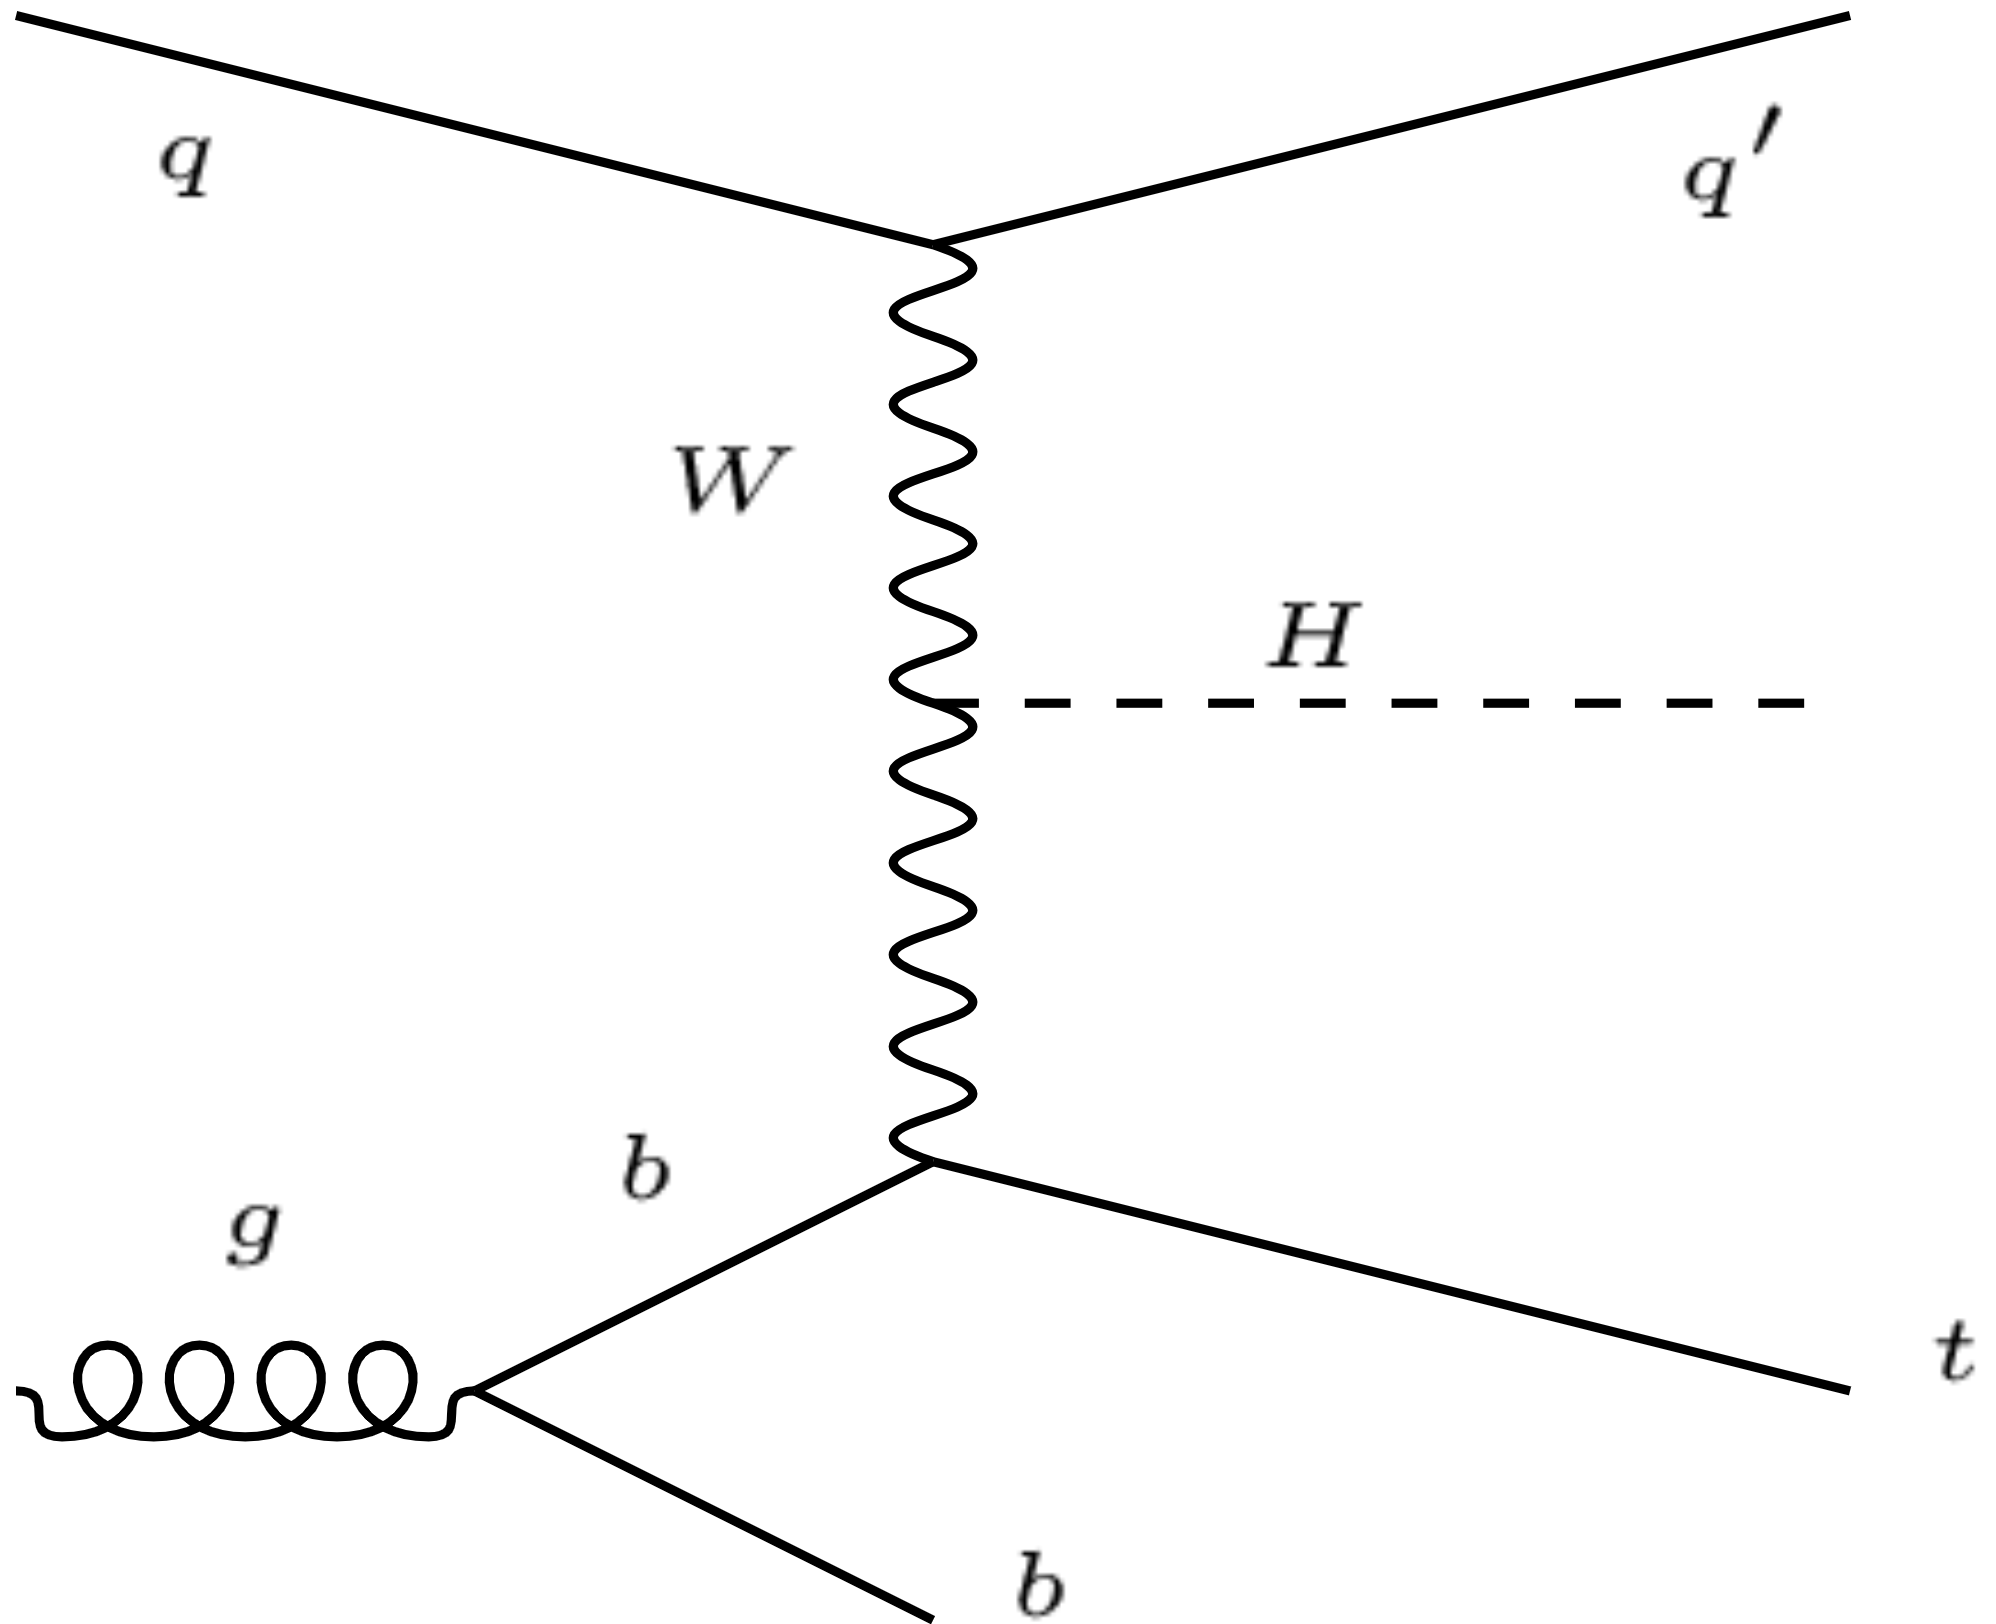
\includegraphics[width=.5\textwidth]{Feynman_diagrams/old/tChnnnael_tHq_H_from_W}
\caption{LO Feynman diagram for the \tHq process}
\label{fig:tHq:TruthFeyman:HfromW}
\end{figure}

% B-quarks
\paragraph{\Pbottom quarks}\mbox{}\\
 Afterwards, the second \Pbottom-quark is identified as the one whose parent
 is a gluon since it is originated from the gluon splitting. The \Pbottom-quark originated 
 from the top-quark-decay system is saved as well. In Figure~\ref{fig:tHq:pTvsEta_bQuark}
 the $\pT$ and $\eta$ distributions of these quarks are compared using the truth-level
 information.
 
 
\paragraph{Further decays}\mbox{}\\
Finally, all the possible decays from the Higgs-boson children are considered.
These are further decayed several times to explore all possible final states. %possible final-states
The range of possible combinations is wide and the particular configuration that defines
a final-state channel can be achieved in more than one way. 
%For all \tHq events, the information of
%all particles involved in the event is stored in the NTuples.

%https://gitlab.cern.ch/IFIC-Valencia/tHqIFIC/-/blob/Dileptau/tHqGraphics/thq-truth/4TruthHistos.py
 
 
\begin{comment}
% General features
\paragraph{General Features}\mbox{}\\
The variables associated to the
Higgs boson, top quark and their corresponding decay
products have the following general features:

\begin{itemize}
\item The parton-level truth variables (i.e.\ the ones starting with
  \texttt{MC\_}) are only filled properly when the Higgs
  boson decays to \WW, \ZZ or $\tau\tau$ (except the variable
  \texttt{MC\_H\_decay} which is filled for all events) and when the
  top quark decays into $Wb$.
\item For each variable, there are five branches in the
  \texttt{truth} tree. Their names are the variable name plus one of the following suffixes: \texttt{\_pt}, \texttt{\_eta}, \texttt{\_phi}, \texttt{\_m} and
  \texttt{\_pdgId}. Some of the $\tau$ related variables have the \texttt{\_isHadronic} suffix. 
\item The \texttt{\_isHadronic}-type variables refer only to $\tau$ particles
  and they store wether the $\tau$ decays hadronically or leptonically. 
  If the $\tau$ decays to a light lepton, it stores the PDG-ID of that lepton
  and if it decays hadronically it stores the PDG-ID of the \PWm for $\tau^-$ 
  and  the \PWp for $\tau^+$.
\item The default value is \(-1000\) for the branches ending with \texttt{\_pt},
  \texttt{\_eta}, \texttt{\_phi} , \texttt{\_m} while -9999 is the
  default value for the ones ending with \texttt{\_pdgId} and \texttt{\_isHadronic}. 
\item For Higgs-boson decays, \texttt{\_decay1\_} stores particles with positive PDG-ID
  while \texttt{\_decay2\_} stores particles with negative PDG-ID.
\item Unless stated otherwise, we are storying the particles after the final state  radiation (FSR) \textit{i.e.} right before decaying. %Review how accurate is this
%   \item For the decay products of the $W/Z$ bosons and $\tau$'s, \texttt{\_decay1\_} is used to store either hadron or
%   lepton information (generally with negative PDF-ID) while
%   \texttt{\_decay2\_} is used for the either neutrino or the lepton information (generally with positive PDG-ID).
\end{itemize}
\end{comment}

%\paragraph{Results}\mbox{}\\
 %\pablo{Pie charts from TopPartons info}

 
 % Scripts: 
%.  https://gitlab.cern.ch/atlas/athena/-/blob/21.2/PhysicsAnalysis/TopPhys/xAOD/TopPartons/Root/CalcThqPartonHistory.cxx
%.  https://gitlab.cern.ch/atlas/athena/-/blob/21.2/PhysicsAnalysis/TopPhys/xAOD/TopPartons/Root/PartonHistoryUtils.cxx


%%%%%%%%%%%%%%%%%%%%%%%%%%%%%%
%           Calculations of expected parton level   results      %
%%%%%%%%%%%%%%%%%%%%%%%%%%%%%%
\section{BR-based calculation for the \tHq fractions}
\label{sec:ChaptH:Sig:truth:Calculations}
%\paragraph{Calculations}\mbox{}\\
 On the other side, the BR-based calculations are used to determine the fraction of each decay channel that is present in the \dileptau. This predictions should be match the fractions obtained with \texttt{TopPartons}. I performed this 
calculations to validate the code
not only for the \dileptau channels but also for the $3\ell$.  By doing so, even a further confirmation
of the proper functioning of the code is achieved. 
For the calculations, the 
BRs of the three Higgs-boson-decay modes that are considered are~\cite{Workman:2022ynf}:
\begin{itemize}
	\item  BR(\Htautau)$= 56.65\%$
	\item  BR(\HWW)$= 5.12\%$ 
	\item  BR(\ZZ)$= 37.43\%$
\end{itemize}
The decay products of each pair of Higgs-boson children are combined and the total decay fractions of %total decay-fractions
these combinations are computed. To do so, the following decay ratios are used~\cite{Workman:2022ynf}:

\begin{multicols}{2}
For the \Ptau leptons 
\begin{itemize}
	\item  BR($\tau \rightarrow \Pe \Pnu \Pnu)= 17.82\%$
	\item  BR($\tau \rightarrow \Pmu \Pnu \Pnu)= 17.39\%$
	\item  BR($\tau \rightarrow$ Hads.)$= 64.74\%$
\end{itemize}
\columnbreak
For the \PW bosons
\begin{itemize}
	\item  BR($\PW \rightarrow \Pe \Pnu) = 10.71\%$
	\item  BR($\PW \rightarrow \Pmu \Pnu) = 10.63\%$
	\item  BR($\PW \rightarrow \Ptau \Pnu) =11.38\%$
	\item  BR($\PW \rightarrow$ Hads.)$= 67.41\%$
\end{itemize}
\end{multicols}
For the \PZ bosons
\begin{itemize}
	\item  BR($\PZ \rightarrow \Pe \Pe)= 3.36\%$
	\item  BR($\PZ \rightarrow \Pmu \Pmu)= 3.36\%$
	\item  BR($\PZ \rightarrow \Ptau \Ptau)= 3.36\%$
	\item  BR($\PZ \rightarrow \Pnu \Pnu)= 20\%$
	\item  BR($\PZ \rightarrow$ Hads.)$= 69.91\%$
\end{itemize}

Note that the BRs of the considered decay modes are normalised
so that its sum is the 100\% ~\cite{Workman:2022ynf}.
If the \PW or \PZ decays to a \Ptau, it is further decayed into either
a $\emu$ or \tauhad. 
For each of the Higgs-boson-decay modes, the possible final states are studied %possible final-states
and its correspondent fractions are calculated. 

For \Htautau:
\begin{itemize}
	\item  BR($\tautau \rightarrow \emu + \emu)= 12.41\%$
	\item  BR($\tautau \rightarrow \emu + \tauhad)= 45.63\%$
	\item  BR($\tautau \rightarrow$ Hads.)$= 41.51\%$
\end{itemize}

For \HWW the first two elements of the list take part 
in the \dileptau signature when the \tauhad comes from 
the \Ptop quark in the first item and the \PHiggs boson
in the second. 
\begin{itemize}
	\item  BR($\WW \rightarrow \emu +\emu)= 6.42\%$ 
	\item  BR($\WW \rightarrow \emu +\tauhad)= 3.73\%$
	\item  BR($\WW \rightarrow \emu$ +$\,$Hads.$)= 34.17\%$
	\item  BR($\WW \rightarrow$ Hads.)$= 55.92\%$
\end{itemize}

For the \ZZ the $\ZZ \rightarrow 2 \times \emu$ contributes 
to the \dileptau signature when the \tauhad is produced in the
top-quark system. When the top quark decays into a 
light lepton, the $\ZZ \rightarrow \emu + \tauhad$ mode contributes
to the \dileptau final state.
\begin{itemize}
	\item  BR($\ZZ \rightarrow 4 \times \emu)= 0.52\%$ 
	\item  BR($\ZZ \rightarrow 2 \times \emu)= 12.85\%$
	\item  BR($\ZZ \rightarrow \emu +\tauhad)= 12.85\%$
	\item  BR($\ZZ \rightarrow 4 \times \nu$+Hads.$)= 80.82\%$
	\item  BR($\ZZ \rightarrow 2 \times \tauhad)= 2.82\%$	
	\item  BR($\ZZ \rightarrow 3 \times \emu + \tauhad)= 0.22\%$
\end{itemize}


For the top-quark system only the $\Ptop \rightarrow \PW + \Pbottom$
mode is taken into account and the \PW boson is further decayed until there are
either hadrons, light leptons or a \tauhad. Except when the \PW decays directly
into hadrons, all modes contribute to the \dileptau channel.


Combining all the decay modes presented brings out a wide variety of final states 
with different probabilities. For the \dileptau final state, these results are summarised in
Table~\ref{tab:ChaptH:TruthSummary}. % and Figure~\ref{fig:tHq:Truth:PieChartHiggsDecayModes}.
Additionally, from these calculations can be deduced that from all \tHq events, only
a $3.72\%$ decay into a \dileptau final state. %  dileptau = 3.715767739%
From these, in more than 80\% of cases the \tauhad is produced in
the Higgs-boson-decay chain.


% Describir los cálculos que hay aquí https://docs.google.com/spreadsheets/d/1e5kLqJrDCyxE28ecdznN4IDwZtDTQz0pQHcXfehRsYM/edit#gid=0
	

%\begin{figure}[htbp!]
%\centering
%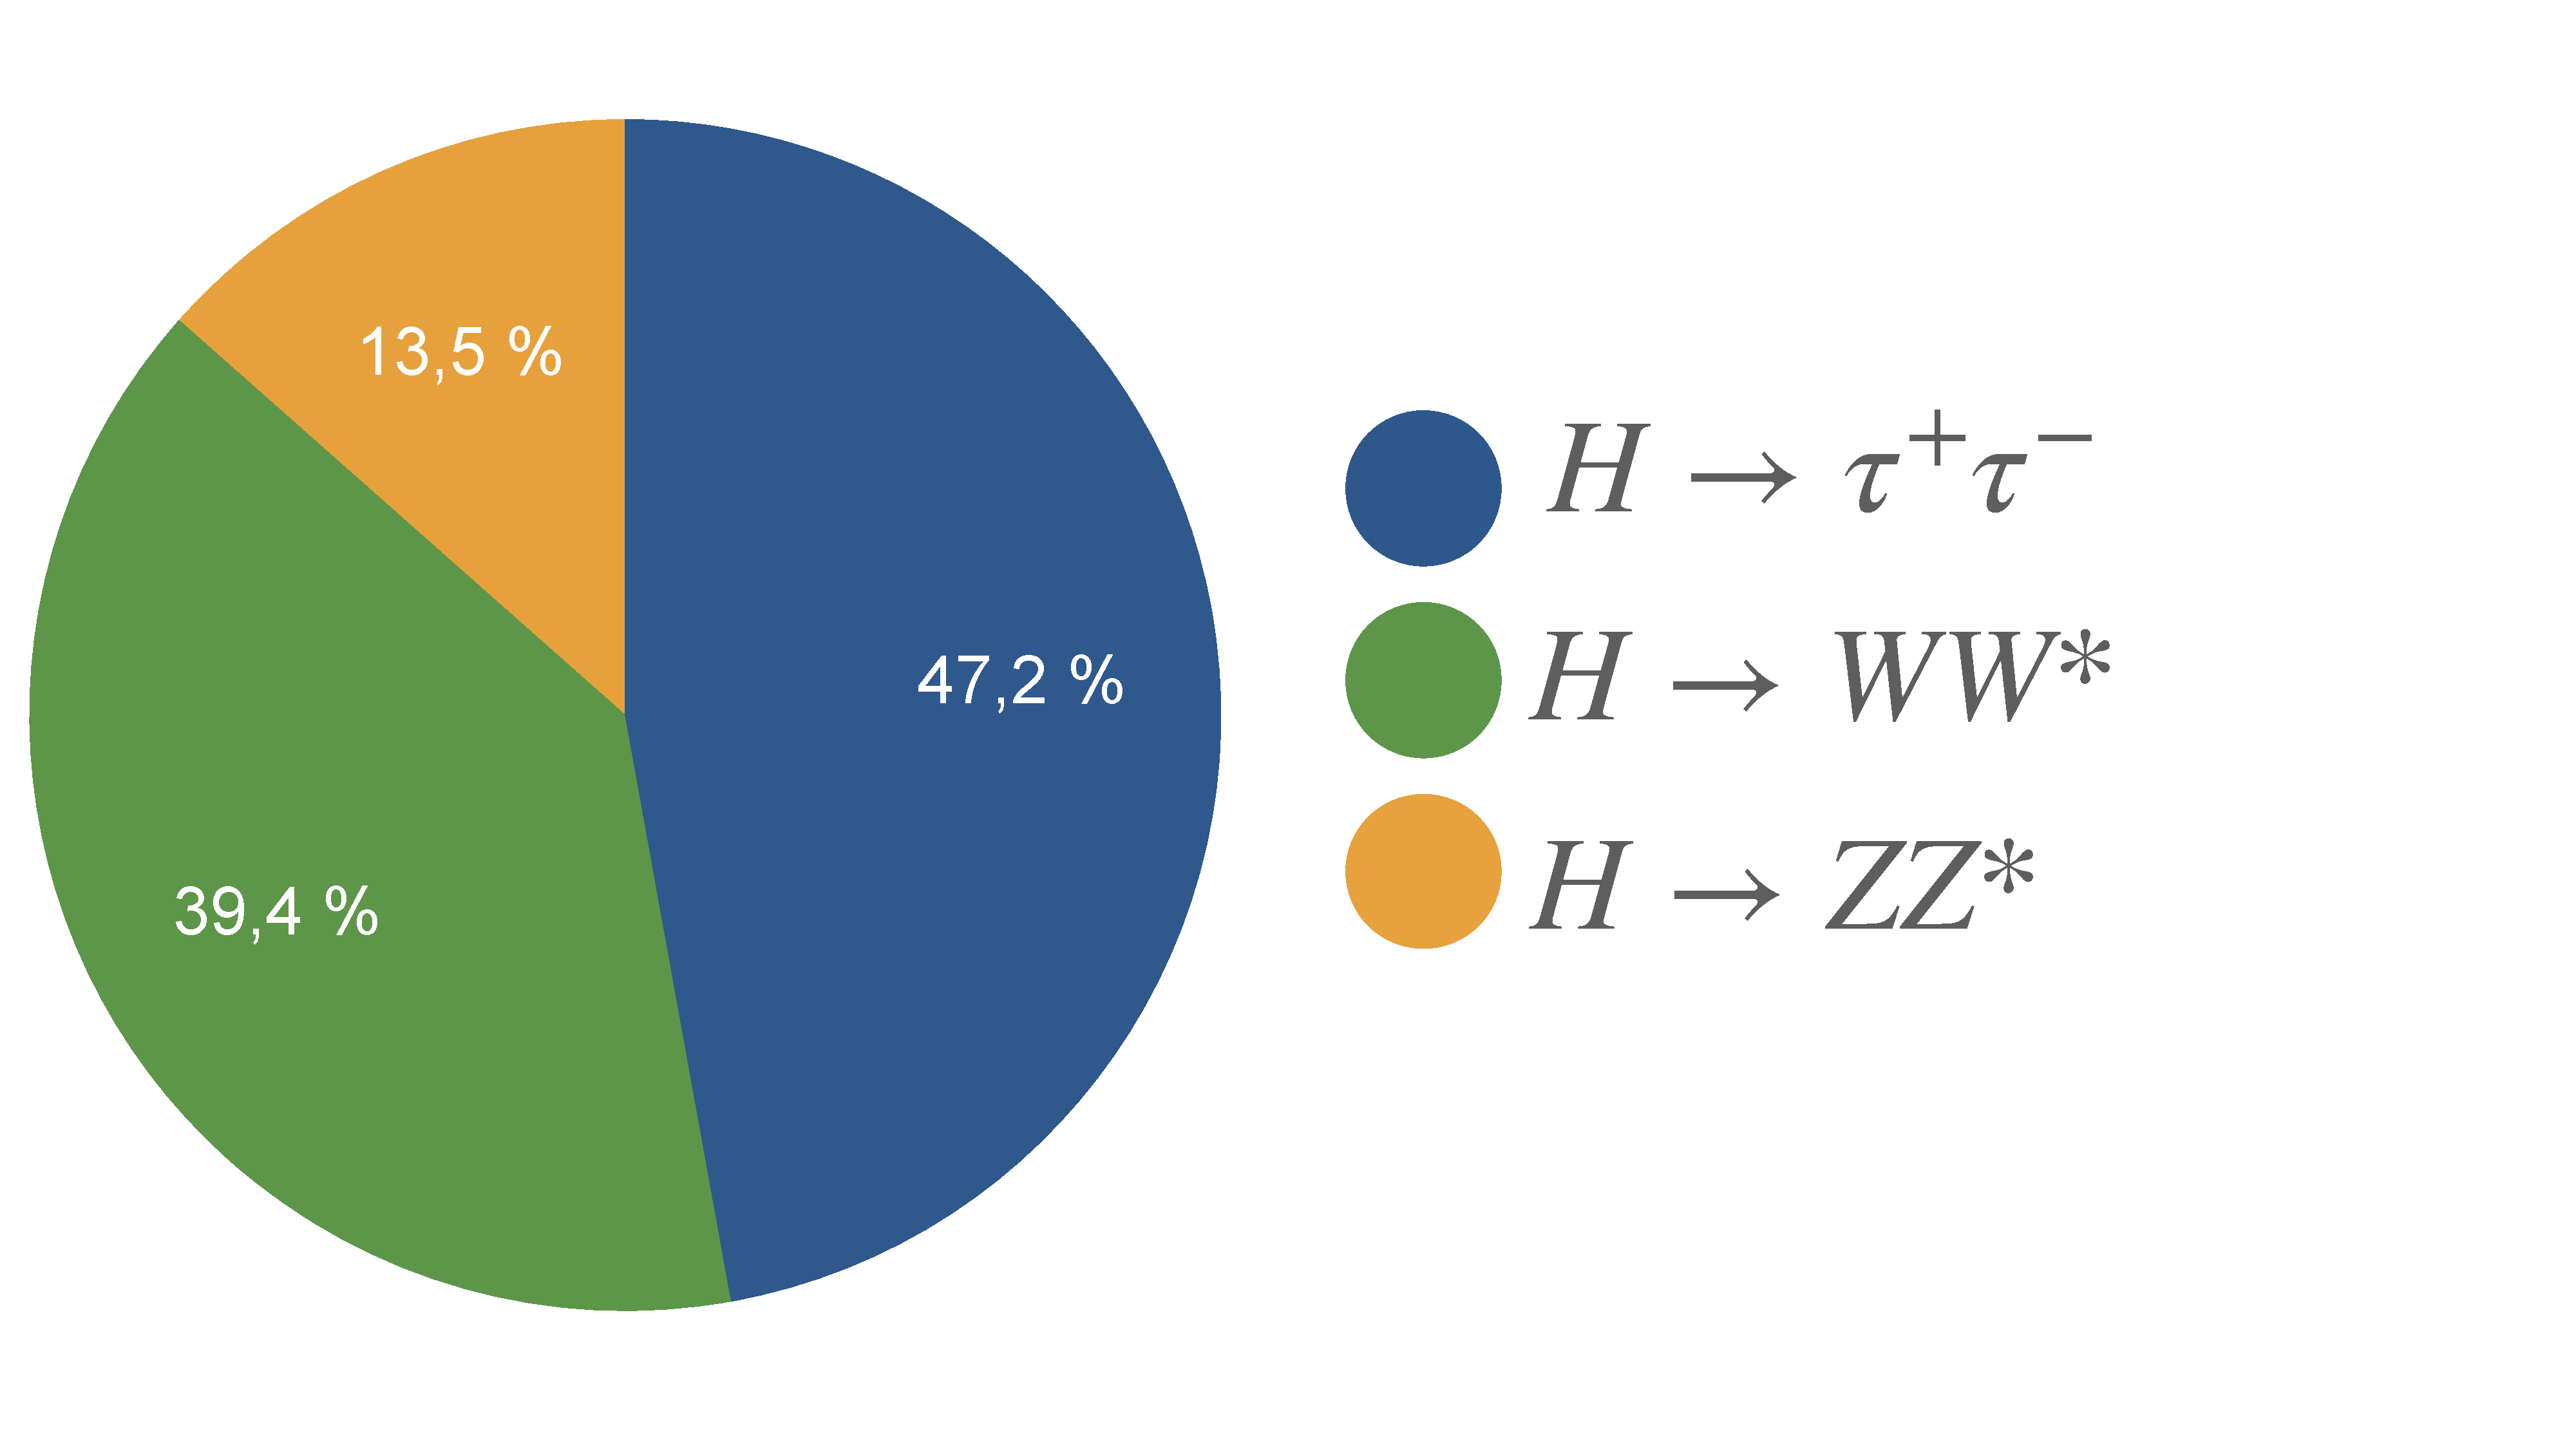
\includegraphics[width=.75\textwidth]{Chapter5_tHq/PieChartHiggsDecayModes}
%\caption{Relative contribution of each Higgs-decay channel to the \dileptau final state. Results obtained from theoretical 
%calculations. \pablo{este pie chart está mal}}
%\label{fig:tHq:Truth:PieChartHiggsDecayModes}
%\end{figure}


%> truth = generator + parton shower + hadronisation
%> The studies I did were done at generator level
%> Particle level is part of truth information
%> Detector level = reconstruction level + calibration + 

%source: https://docs.google.com/spreadsheets/d/1e5kLqJrDCyxE28ecdznN4IDwZtDTQz0pQHcXfehRsYM/edit#gid=0

